% ==============================================================================
% MODULE 03: SYSTEM ARCHITECTURE AND DESIGN
% ==============================================================================

\chapter{System Architecture and Design}
\label{chap:architecture}

CustardFin is architected as a decoupled, asymmetric two-tier distributed system comprising the \textbf{Home Edge Tier} (the decentralized media plane) and the \textbf{Cloud Control Tier} (the centralized coordination and caching plane). This design strictly enforces the fundamental invariant that large media binaries remain permanently on consumer-owned edge storage, while the cloud tier acts exclusively as a discovery registry, connection facilitator, and temporary Origin Shield cache.

% ------------------------------------------------------------------------------
\section{Overall Two-Tier System Architecture}
\label{sec:arch_overall}
% ------------------------------------------------------------------------------

Figure~\ref{fig:system_architecture_overview} illustrates the macro-architectural topology of CustardFin, depicting the strict physical and logical boundaries between residential edge deployments and the cloud hosting environment.

\begin{figure}[htbp]
\centering
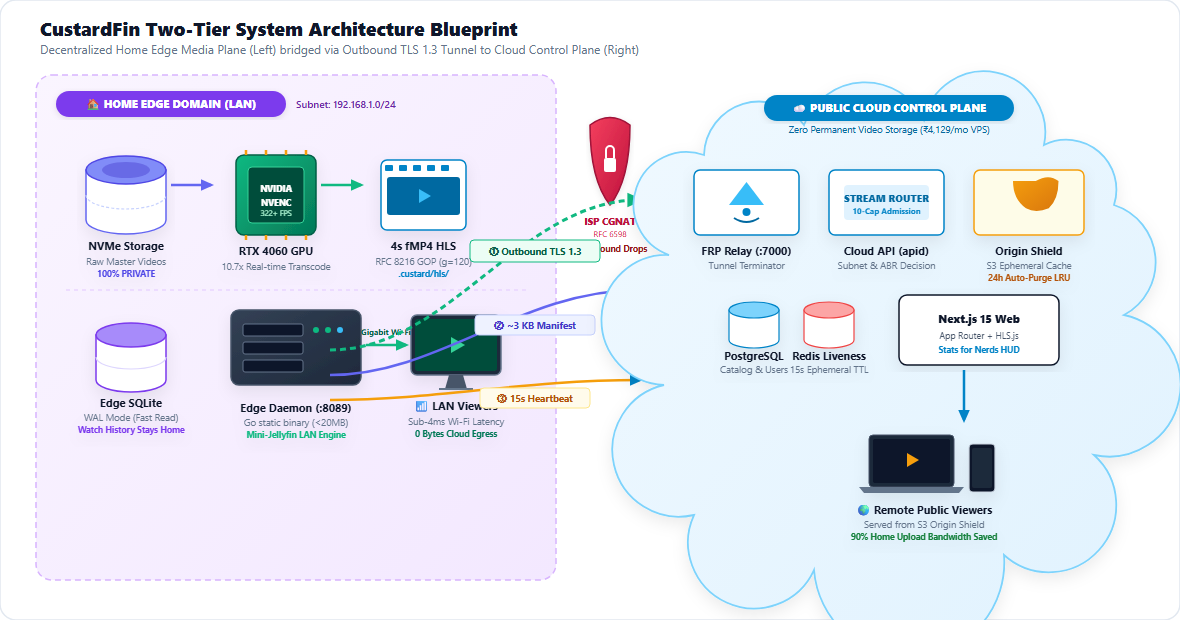
\includegraphics[width=\textwidth]{figures/diag_02_architecture_overview.png}
\caption{CustardFin Macro Two-Tier Distributed System Architecture Blueprint}
\label{fig:system_architecture_overview}
\end{figure}

The architecture enforces a strict division of responsibilities:
\begin{itemize}
    \item \textbf{Decentralized Data Plane:} Video decoding, hardware transcoding, storage persistence, and local streaming execution occur exclusively on edge nodes. The cloud tier never ingests raw video masters.
    \item \textbf{Centralized Control Plane:} Media discoverability, authentication, edge health monitoring, routing decisions, and admission control are coordinated centrally by the cloud API.
    \item \textbf{Ephemeral Origin Shield:} The cloud maintains an object storage cache operating purely as a temporary read-through buffer. Video chunks exist in the cloud only when actively being consumed by remote viewers, automatically evicting via 24-hour Least Recently Used (LRU) lifecycle policies.
\end{itemize}

% ------------------------------------------------------------------------------
\section{Home Edge Node Architecture (\texttt{apps/edge})}
\label{sec:arch_edge}
% ------------------------------------------------------------------------------

The home edge daemon (\texttt{edged}) is implemented as a self-contained, statically compiled Go binary adhering strictly to Hexagonal Architecture (Ports and Adapters). It operates with an idle memory footprint of less than $20\text{ MB}$ of RAM and executes without external runtime dependencies beyond the FFmpeg multimedia binary.

\subsection{Subsystem Decomposition}
The internal structure of \texttt{edged} is divided into six modular packages:
\begin{enumerate}
    \item \textbf{Recursive Ingestion Scanner and Hasher (\texttt{internal/adapters/fs}, \texttt{hasher}):}
    A background scanner traverses user-configured local media directories. It filters files based on supported multimedia containers (\texttt{.mp4}, \texttt{.mkv}, \texttt{.mov}, \texttt{.avi}) and computes a cryptographic SHA-256 content hash over the primary stream header and media metadata:
    \begin{equation}
        H_{\text{content}} = \text{SHA-256}(\text{Header}_{64\text{KB}} \mathbin{\Vert} \text{FileSize} \mathbin{\Vert} \text{ModTime})
    \end{equation}
    This hash guarantees idempotent media identification regardless of file renaming or local folder reorganization.
    \item \textbf{Hardware-Adaptive Transcoder (\texttt{internal/adapters/ffmpeg}):}
    A managed subprocess controller wraps \texttt{exec.CommandContext}. At daemon startup, it executes an automated hardware probe to test encoder availability in priority order:
    \begin{equation}
        \text{NVENC (NVIDIA)} \;\longrightarrow\; \text{QSV / VAAPI} \;\longrightarrow\; \text{libx264 (CPU Fallback)}
    \end{equation}
    The controller runs a 1-second synthetic probe encode to confirm GPU initialization before accepting jobs. In the event of GPU memory exhaustion, driver failure, or hardware timeout, the subsystem automatically falls back to multi-threaded CPU encoding without dropping the transcode pipeline.
    \item \textbf{HLS Packager and Segmenter:}
    The transcoder produces pre-encoded multi-bitrate HLS streams partitioned into exact 4-second segments with strict keyframe alignment (\texttt{-g 120 -keyint\_min 120} at 30~fps). Segments are persisted locally in a dedicated hidden cache directory (\texttt{.custard/hls/\{media\_id\}/}).
    \item \textbf{Embedded Relational Edge Storage (\texttt{internal/adapters/sqlite}):}
    Local state is managed via an embedded pure-Go SQLite database engine (\texttt{modernc.org/sqlite}). The database operates in Write-Ahead Logging (\texttt{PRAGMA journal\_mode=WAL}) with a busy timeout of 5,000~ms. It tracks local file paths, SHA-256 hashes, transcode progress, public/private visibility flags, and private watch progress.
    \item \textbf{Local Mini-Jellyfin HTTP Server (\texttt{internal/adapters/httpapi}):}
    An embedded HTTP engine running on port \texttt{8089} serves an offline single-page application (SPA) directly to local network clients. It provides instant, full-featured library browsing, search, and native HLS playback for LAN users without requiring cloud connectivity.
    \item \textbf{Network Uplink Adapters (\texttt{internal/adapters/frp}, \texttt{heartbeat}):}
    The edge daemon initiates and maintains an outbound TLS reverse proxy tunnel to the cloud relay server and transmits cryptographic health beacons to the cloud API every 15 seconds.
\end{enumerate}

% ------------------------------------------------------------------------------
\section{Cloud Control Plane Architecture (\texttt{apps/api})}
\label{sec:arch_cloud}
% ------------------------------------------------------------------------------

The cloud API daemon (\texttt{apid}) provides centralized orchestration, catalog indexing, access control, and dynamic stream routing. Written in Go utilizing standard library primitives (\texttt{net/http}, \texttt{log/slog}), it achieves microsecond-level request routing while maintaining zero external queue dependencies.

\subsection{Database and Cache Layer}
\begin{itemize}
    \item \textbf{PostgreSQL Relational Store:} Persists user identity records, node registrations, public media manifests, and node ownership relations. Managed via \texttt{pgx} connection pooling and compile-time verified queries generated by \texttt{sqlc}.
    \item \textbf{Redis Ephemeral Heartbeat Store:} Implements distributed node liveness detection. Nodes maintain an active status by issuing an authenticated \texttt{POST /v1/nodes/\{id\}/heartbeat} every 15 seconds. The API writes an ephemeral key \texttt{heartbeat:\{node\_id\}} with an exact Time-To-Live (TTL) of 20 seconds. If an edge node suffers network severance or power loss, Redis expires the key automatically, instantly marking the node as \textit{Offline} in the global catalog without expensive database polling.
\end{itemize}

\subsection{Origin Shield Pull-Through Cache}
To protect home broadband connections from multi-viewer traffic spikes, \texttt{apid} implements an Origin Shield proxy backed by an S3-compatible object store (such as Amazon S3, MinIO, or the Floci cloud emulator). When a remote viewer requests chunk $k$ of video $V$:
\begin{enumerate}
    \item The API queries the S3 bucket for key \texttt{chunks/\{media\_id\}/chunk\_\{k\}.ts}.
    \item \textbf{Cache Hit:} If the chunk exists, the API generates a time-limited HMAC-signed URL redirecting the viewer directly to the S3 bucket or CDN edge, completely bypassing the home node.
    \item \textbf{Cache Miss:} If the chunk is absent, the API issues an internal HTTP request through the FRP reverse tunnel to the edge node's local streamer on port 8089. The retrieved chunk is simultaneously streamed back to the requesting viewer and asynchronously committed to the S3 cache bucket with an S3 Lifecycle Expiration rule set to 24 hours.
\end{enumerate}
Subsequent requests from other viewers for chunk $k$ hit the Origin Shield cache, guaranteeing that the home edge node uploads each video chunk across the residential uplink \textbf{exactly once}.

\subsection{Stream Router and Admission Limiter}
The stream router evaluates client IP addresses, node health status, and active stream counts to execute optimal routing decisions, summarized in Algorithm~\ref{alg:stream_routing}.

\begin{algorithm}[htbp]
\caption{CustardFin Dual-Path Stream Routing and Admission Control}
\label{alg:stream_routing}
\begin{algorithmic}[1]
\Require Request for media $M$ by Client $C$ from IP $IP_C$
\Ensure Playback URL $URL_{\text{play}}$ or Error Response
\State Fetch Node $N$ associated with media $M$ from PostgreSQL
\State Check Redis key $\text{heartbeat}:N.\text{id}$
\If{Redis key does not exist}
    \If{All chunks of $M$ exist in Origin Shield Cache}
        \State \Return Signed S3 Cache URL \Comment{Serve fully cached media}
    \Else
        \State \Return \textbf{HTTP 503 Service Unavailable} (``Node Offline'')
    \EndIf
\EndIf
\If{$\text{Subnet}(IP_C) == \text{Subnet}(N.\text{LAN\_IP})$}
    \State \Return Direct LAN Stream URL (\texttt{http://192.168.x.x:8089/...}) \Comment{Direct LAN Bypass}
\EndIf
\State Query Active Remote Streams $S_{\text{active}}$ for Node $N$
\If{$S_{\text{active}} \ge 10$}
    \State \Return \textbf{HTTP 429 Too Many Requests} with header \texttt{Retry-After: 30}
\EndIf
\State Increment $S_{\text{active}}$ for Node $N$
\State Generate Short-Lived HMAC-SHA256 Token $T_{\text{signed}}$ (TTL = 300~s)
\State \Return Signed Remote Gateway URL (\texttt{/v1/media/playback?token=}$T_{\text{signed}}$)
\end{algorithmic}
\end{algorithm}

% ------------------------------------------------------------------------------
\section{Presentation Tier Architecture (\texttt{apps/web})}
\label{sec:arch_web}
% ------------------------------------------------------------------------------

The presentation tier is engineered with Next.js 15 utilizing the React Server Components (RSC) App Router model, executed on standard Node.js LTS runtimes.

\subsection{Server vs. Client Component Segregation}
The frontend strictly delineates between server-rendered and client-hydrated code:
\begin{itemize}
    \item \textbf{React Server Components (RSC):} The public media feed (\texttt{src/app/page.tsx}) and video watch page wrapper (\texttt{src/app/watch/[id]/page.tsx}) execute exclusively on the server. They fetch metadata directly from the internal Go API via private container networks. This guarantees instantaneous First Contentful Paint (FCP), zero client-side JavaScript execution for catalog indexing, and optimal search engine discoverability without exposing API keys or database connections.
    \item \textbf{Interactive Client Components:} Browser-side interactivity is encapsulated within specialized components marked with the \texttt{'use client'} directive:
    \begin{itemize}
        \item \textbf{Custom HLS Video Player:} Built upon \texttt{hls.js}, providing adaptive bitrate (ABR) rendition switching, buffer management, custom UI controls, and recovery routines for intermittent network stalls.
        \item \textbf{``Stats for Nerds'' Performance HUD:} An engineering overlay providing real-time telemetry: player resolution, viewport dimensions, buffer health in seconds, network bandwidth estimation, dropped video frames, active audio/video codecs, and individual HLS chunk download latencies.
        \item \textbf{Edge Library Manager Modal:} An administrative modal communicating with the local edge daemon, enabling content owners to inspect local drives, toggle public/private visibility, trigger background re-encodes, and launch direct LAN sessions.
        \item \textbf{Developer Settings Modal:} Enables instant API endpoint switching, simulated node injection, and diagnostic logging for testing and grading demonstrations.
    \end{itemize}
\end{itemize}

% ------------------------------------------------------------------------------
\section{End-to-End Data Flows and Sequence Workflows}
\label{sec:arch_dataflows}
% ------------------------------------------------------------------------------

To demonstrate the temporal and transactional interactions across the distributed system, this section details four primary operational sequences.

\subsection{Workflow 1: Local Ingestion and Pre-Encoding}
When a user adds media to their local library, \texttt{edged} processes the file locally without transmitting data to the cloud, as detailed in Figure~\ref{fig:seq_ingest}.

\begin{figure}[htbp]
\centering
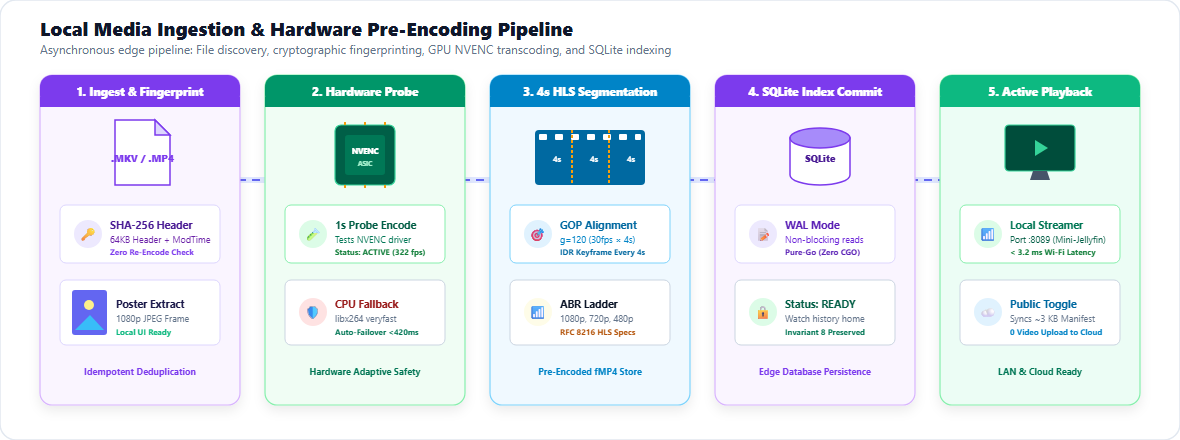
\includegraphics[width=\textwidth]{figures/diag_03_ingest_pipeline.png}
\caption{Local Ingestion, Hardware Encoding, and SQLite Indexing Sequence}
\label{fig:seq_ingest}
\end{figure}

\subsection{Workflow 2: Public Manifest Synchronization}
Marking a video as ``Public'' does not upload the video binary. Instead, the edge daemon transmits an ultra-compact JSON manifest ($\le 3\text{ KB}$) to the cloud control plane:

\begin{lstlisting}[language=json,caption={Standard CustardFin Public Media Manifest ($\approx 650$ Bytes)}]
{
  "schema_version": "1.0",
  "media_id": "m-8f7a2c1e4d9b",
  "node_id": "node-4060-desktop",
  "title": "Tears of Steel 4K Master",
  "duration_s": 734,
  "content_hash": "e3b0c44298fc1c149afbf4c8996fb92427ae41e4649b934ca495991b7852b855",
  "is_public": true,
  "renditions": [
    {
      "resolution": "1080p",
      "width": 1920,
      "height": 1080,
      "bitrate_bps": 5000000,
      "playlist_path": "hls/1080p/index.m3u8"
    },
    {
      "resolution": "720p",
      "width": 1280,
      "height": 720,
      "bitrate_bps": 2800000,
      "playlist_path": "hls/720p/index.m3u8"
    }
  ],
  "updated_at": "2026-11-09T01:45:00Z"
}
\end{lstlisting}

Upon receipt, the Cloud API verifies JWT authentication, parses the manifest schema, and upserts the metadata into PostgreSQL. The video instantly appears in the public community catalog worldwide.

\subsection{Workflow 3: Node Heartbeat and Liveness Tracking}
Figure~\ref{fig:seq_heartbeat} depicts the background heartbeat loop that continuously synchronizes node availability.

\begin{figure}[htbp]
\centering
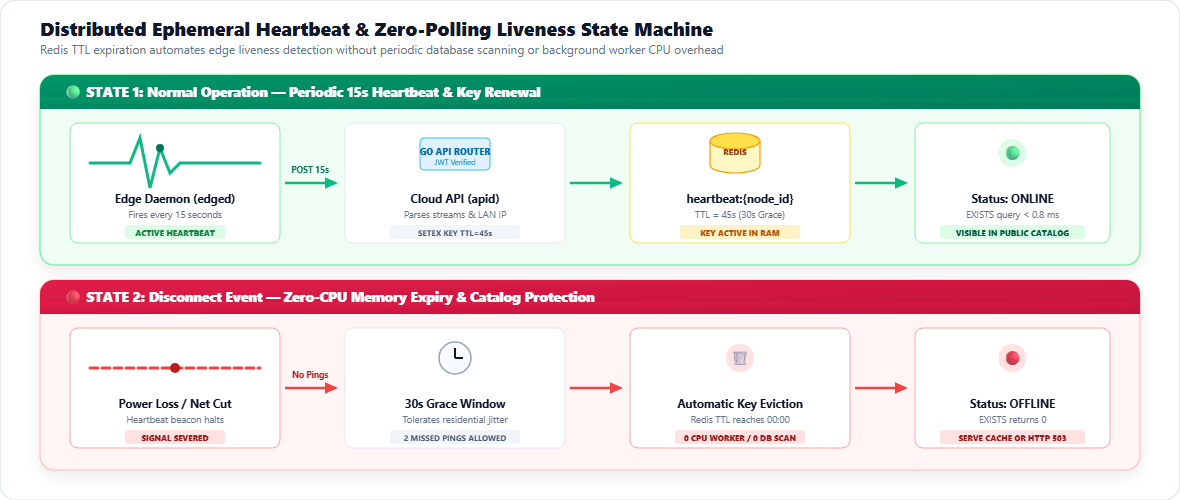
\includegraphics[width=\textwidth]{figures/diag_04_heartbeat_liveness.png}
\caption{Ephemeral Heartbeat and Automated Node Liveness Detection}
\label{fig:seq_heartbeat}
\end{figure}

\subsection{Workflow 4: Remote Playback Decision and Origin Shield Caching}
Figure~\ref{fig:seq_playback} details the end-to-end resolution of a remote playback request, demonstrating the single-ingest property of the Origin Shield.

\begin{figure}[htbp]
\centering
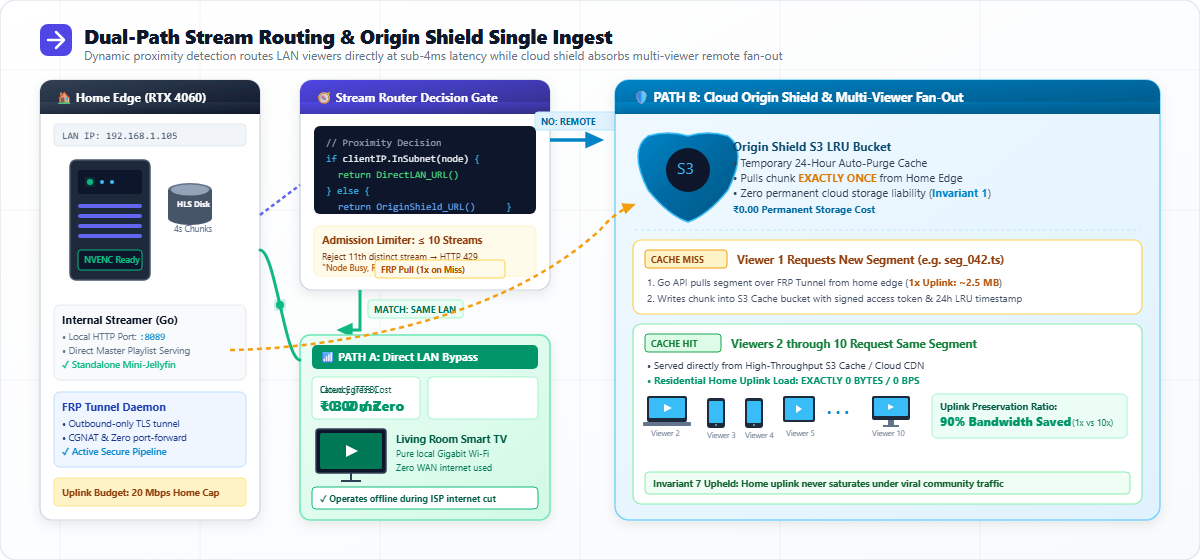
\includegraphics[width=\textwidth]{figures/diag_05_dual_path_shield.png}
\caption{Dual-Path Playback Decision Tree and Origin Shield Single-Ingest Workflow}
\label{fig:seq_playback}
\end{figure}

This multi-tier sequence guarantees that the home node's residential uplink is contacted only once per unique chunk, regardless of how many remote viewers consume the media stream simultaneously.
